\chapter{System Design and Architecture}
\label{chap:design}

\section{System Architecture Overview}
Project FORGE is engineered around a modular, multi-tier decoupled architecture designed to execute on client hardware with zero external runtime dependencies. As illustrated in Figure~\ref{fig:sys_arch}, the game is organized into four layers, and a fifth, offline layer in Python trains and explains the models (Section~\ref{sec:revised_arch}):
\begin{enumerate}
    \item \textbf{Presentation \& Input Layer:} Manages player keyboard/mouse inputs, camera positioning, trauma screen shake, floating combat text, and the real-time supervisor Defense Telemetry Overlay.
    \item \textbf{Core Gameplay Engine Layer (Godot 4.7):} Implements 2D kinematic physics, player state transitions (idle, run, attack, dash), adversary finite state machines, hazard hitboxes, and projectile life-cycles.
    \item \textbf{Generative AI \& Adaptation Layer:} Houses the two-stage dungeon layout generator, the pure-GDScript neural network forward pass (\texttt{PPOPolicy}), and the parameter translation logic (\texttt{DifficultyManager}).
    \item \textbf{Telemetry \& Data Persistence Layer:} Continuously collects fine-grained gameplay metrics, executes cold-start aggregation ($CR_0$), and stores one row per floor in SQLite (JSON fallback).
\end{enumerate}

\begin{figure}[!htbp]
\centering
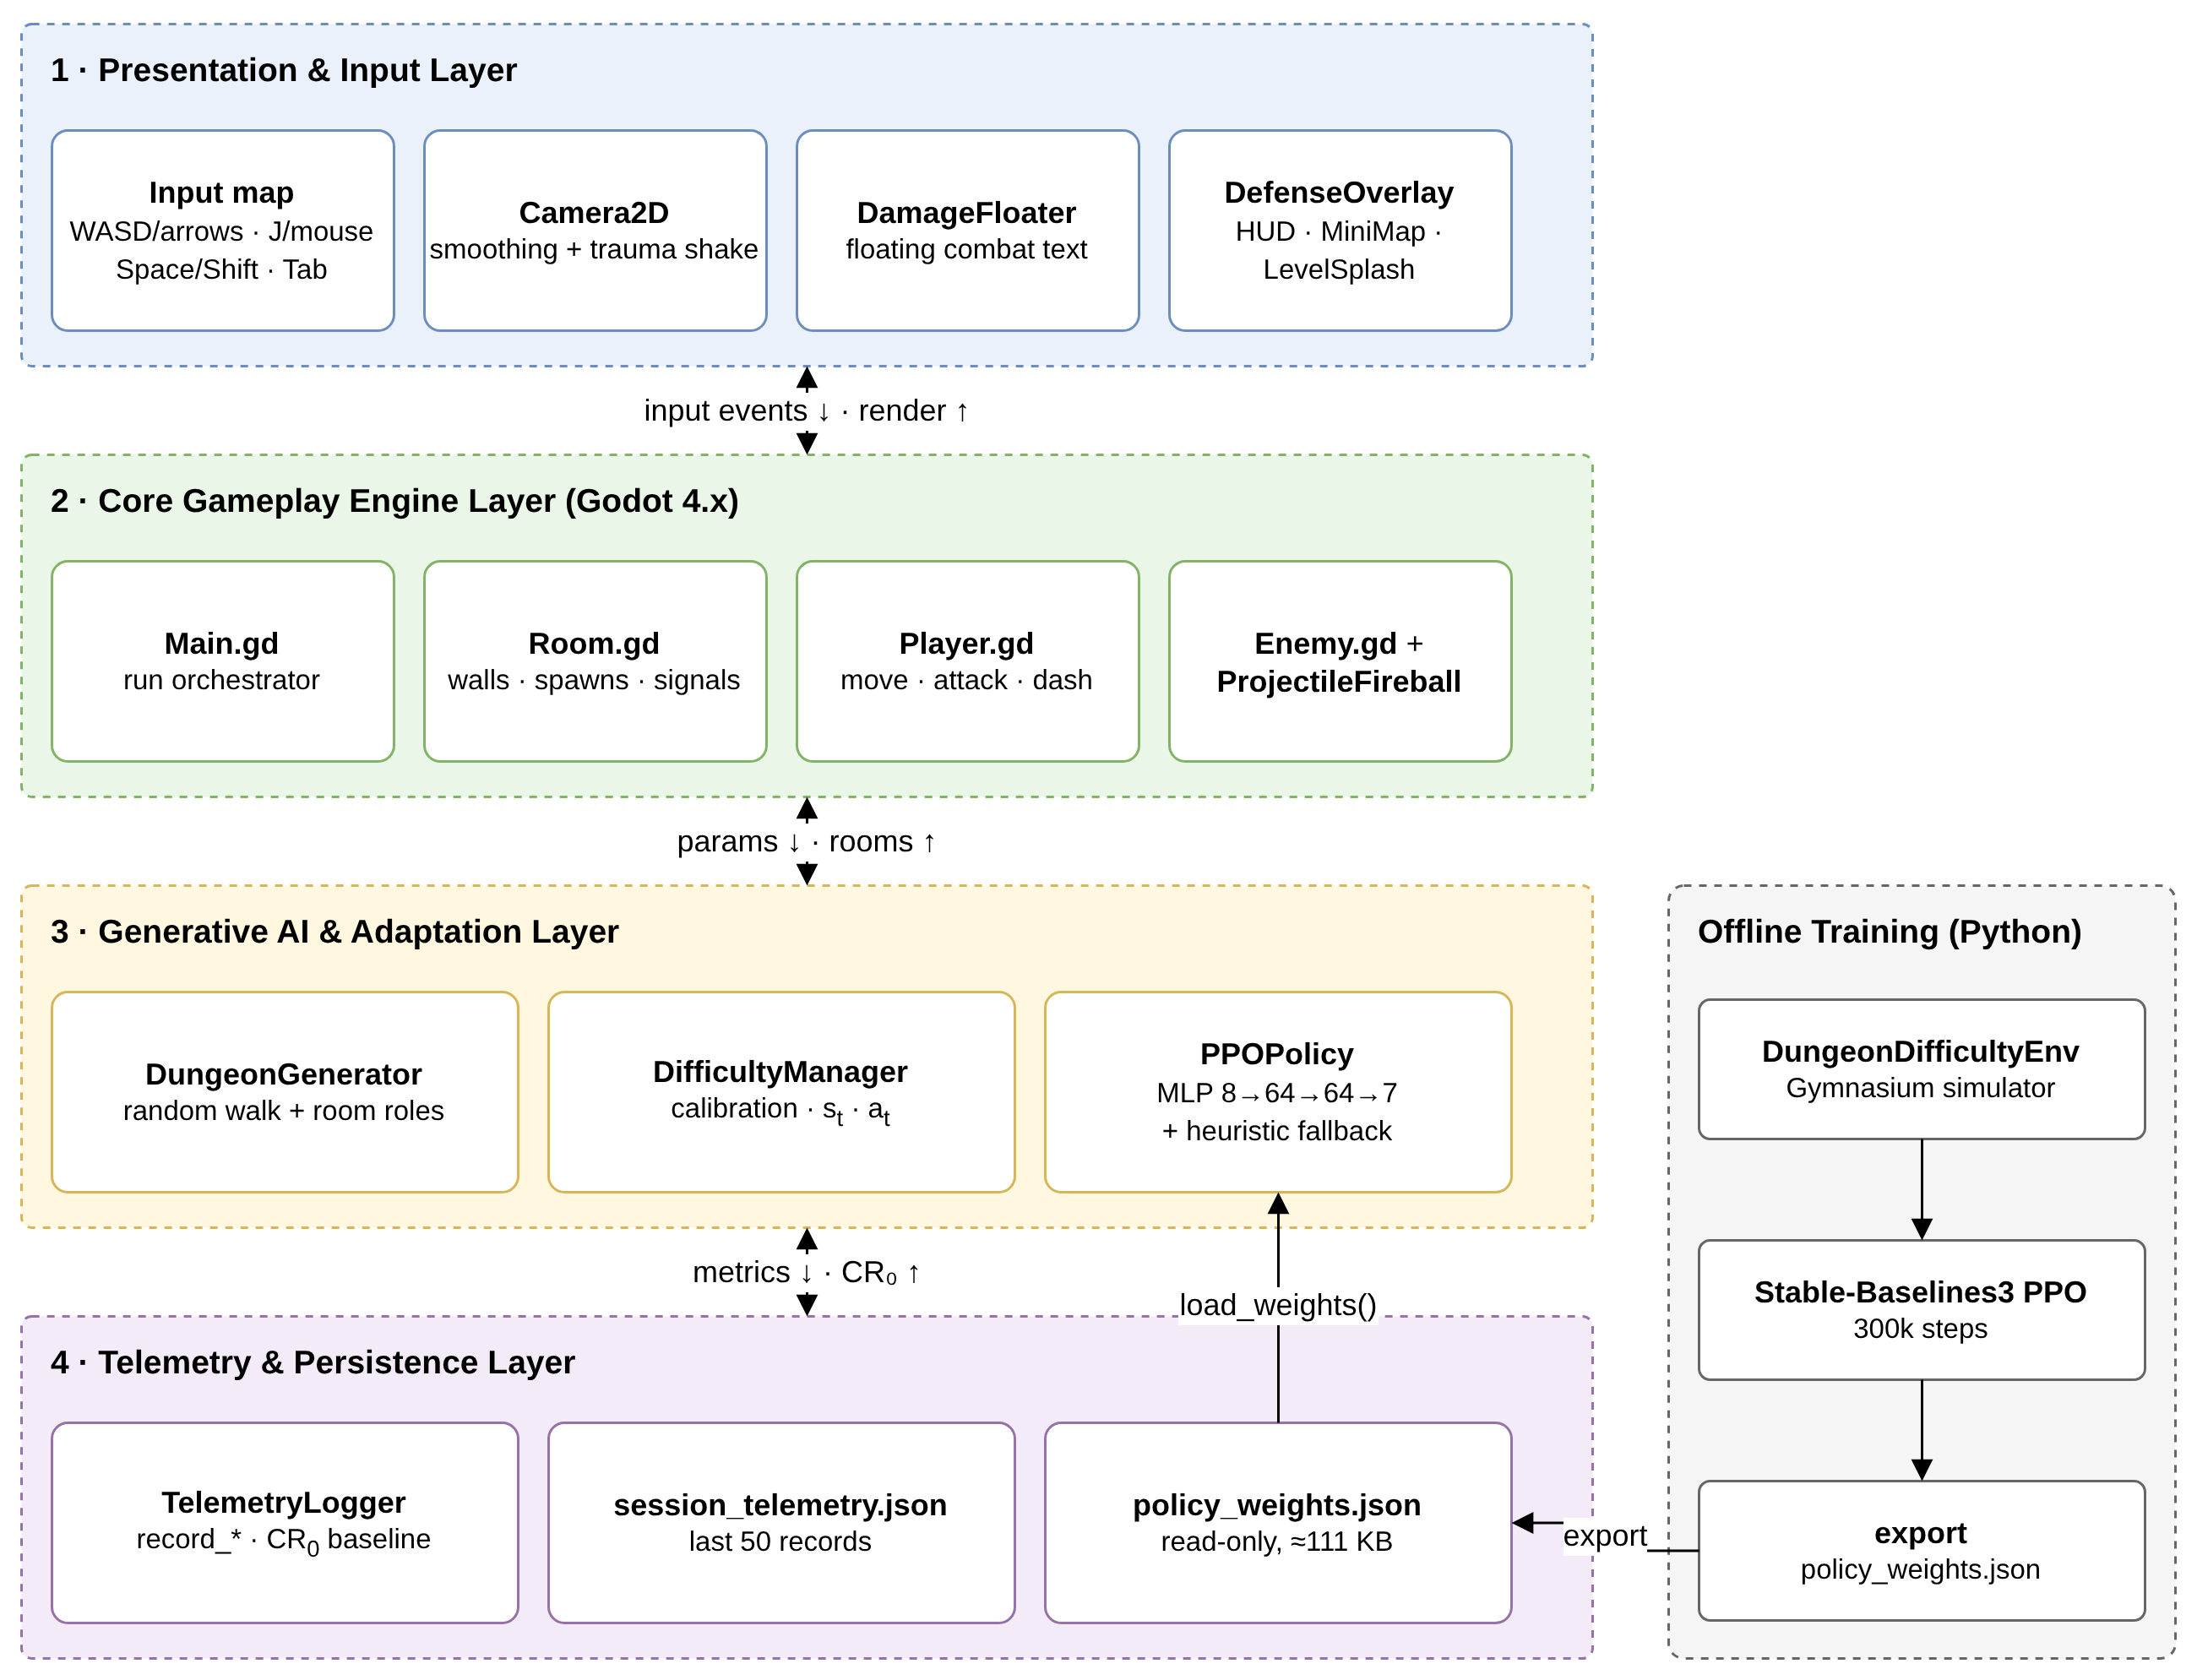
\includegraphics[width=0.95\textwidth]{ThesisFigs/fig_5_1_system_architecture.png}
\caption[Four-Tier System Architecture of Project FORGE]{Four-Tier System Architecture of Project FORGE (Mid-1 drawing; the telemetry layer is now SQLite and the offline layer is shown in Figure~\ref{fig:revised_arch})}
\label{fig:sys_arch}
\end{figure}

\section{Architectural Components}
The primary responsibilities of the core engine components are detailed below:
\begin{itemize}
    \item \textbf{\texttt{Main.gd}:} The central gameplay orchestrator. Coordinates room transitions, scene loading, camera attachment, player death and respawn cycles, trauma camera shake dampening, and inter-floor progression.
    \item \textbf{\texttt{DifficultyManager.gd}:} Acts as the bridge between raw game parameters and the AI policy. Manages the 5-floor cold-start calibration, scales parameters deterministically under Static Baseline mode, normalizes telemetry observations ($s_t$), and denormalizes PPO actions ($a_t$) into concrete bounds.
    \item \textbf{\texttt{DungeonGenerator.gd}:} Executes Stage 1 generation. Generates a grid of rooms by random walk with branching, opens matching doors between neighbouring rooms, picks as the Exit a room at the maximum BFS door depth from the start (ties broken towards rooms not in line with the start), gives each room its own size and corridor length, and assigns the remaining rooms Hazard, Treasure or Combat roles. Because every room is attached to an already placed room, the layout is a connected tree by construction.
    \item \textbf{\texttt{PPOPolicy.gd}:} Contains the neural network forward pass. Loads exported JSON weights, executes the matrix multiplications with $\tanh$ hidden activations in native GDScript, clips the linear output layer to $[-1,1]$ exactly as Stable-Baselines3 does for a deterministic action, and triggers a deterministic heuristic fallback if weights are missing or unparsable.
    \item \textbf{\texttt{TelemetryLogger.gd} and \texttt{telemetry/}:} Operates as an event-driven telemetry sink fed by \texttt{Main.gd}. It writes through a \texttt{TelemetryBackend} interface: \texttt{SqliteBackend} (godot-sqlite, \texttt{schema.sql} with migrations, \texttt{queries.sql}) or \texttt{JsonBackend} as a fallback. Accumulates damage dealt, damage taken, deaths, kills, pickups and hazard hits, and at the end of Floor 5 computes $CR_0$ and the training-scale calibration averages that seed $s_0$.
    \item \textbf{\texttt{Enemy.gd}, \texttt{ProjectileFireball.gd}, \texttt{SlamShockwave.gd}:} The five enemy archetypes (Table~\ref{tab:archetypes}). \texttt{Room.gd} samples an archetype per spawn slot from the current mix.
    \item \textbf{\texttt{ui/ConsentScreen.gd}, \texttt{ui/FloorRating.gd}, \texttt{ui/PauseMenu.gd}, \texttt{GameSettings.gd}, \texttt{BuildInfo.gd}:} Playtest features: consent, the 1--5 rating, pause, and the playtest/dev build split (playtest builds hide the Defense Overlay).
\end{itemize}

Figure~\ref{fig:low_level_arch} illustrates the low-level component interaction and runtime dataflow architecture, capturing the boundary between offline policy synthesis, automated continuous integration verification, and the real-time Godot 4.7 subsystems.

\begin{figure}[!htbp]
\centering
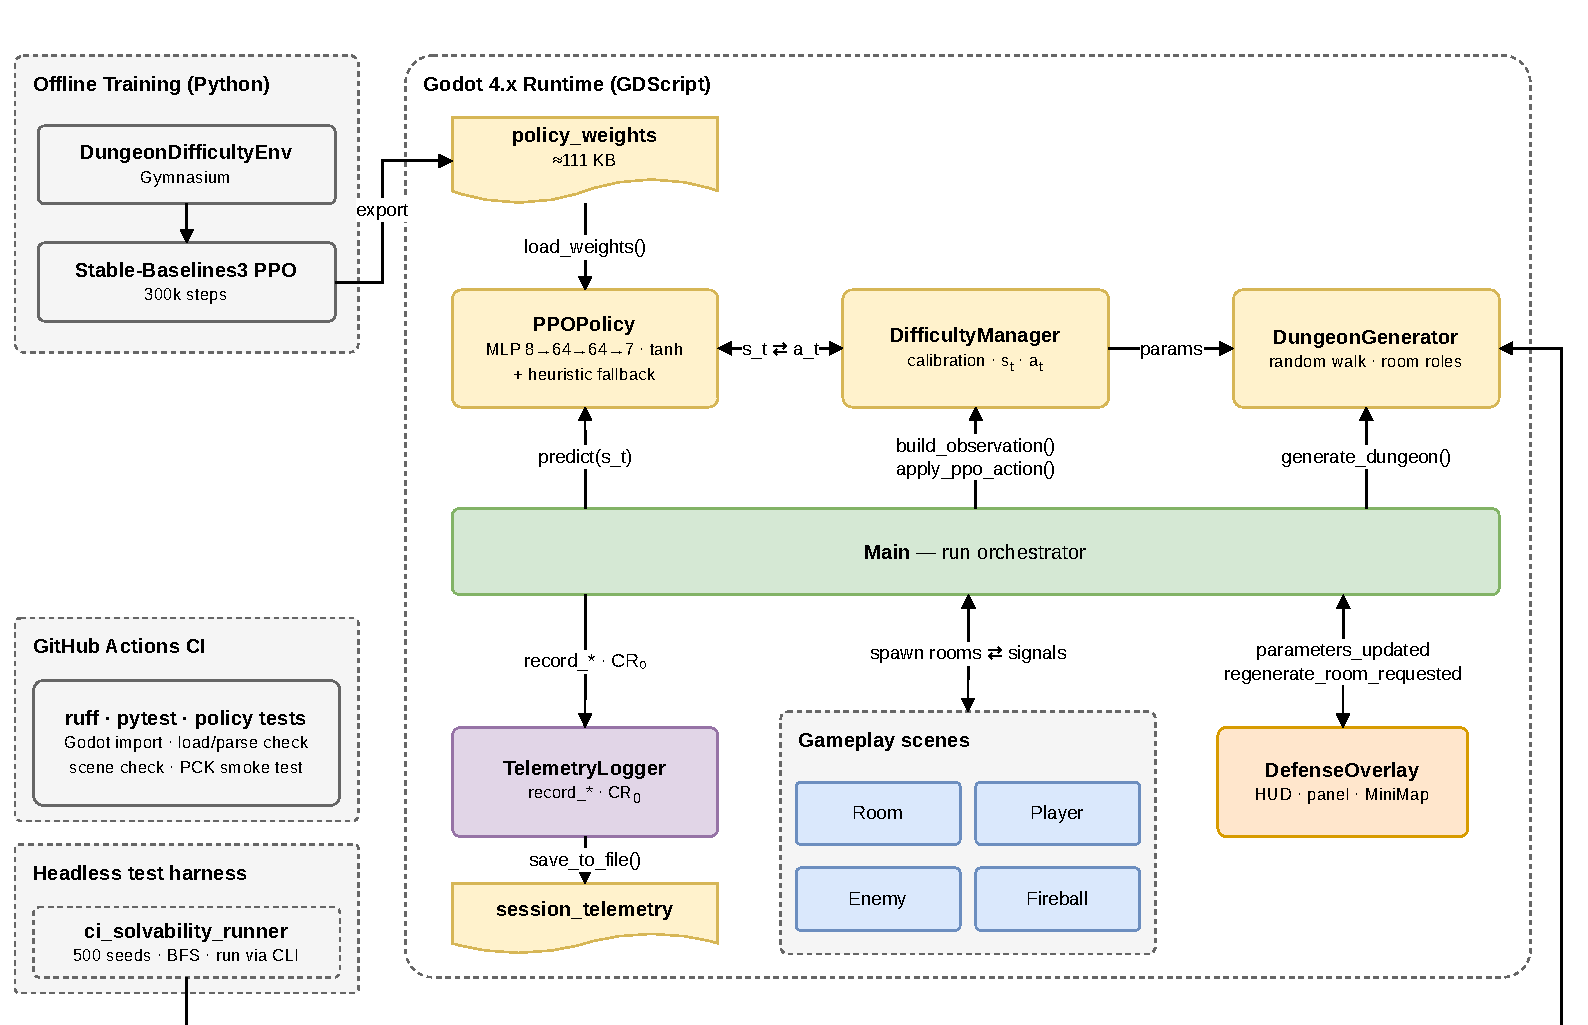
\includegraphics[width=0.95\textwidth]{ThesisFigs/fig_low_level_architecture}
\caption[Low-Level Component Interaction and Runtime Dataflow Architecture]{Low-Level Component Interaction and Runtime Dataflow Architecture (Mid-1 drawing; update pending)}
\label{fig:low_level_arch}
\end{figure}

\section{Interfaces and Data Contracts}

\subsection{Observation Vector Contract ($s_t \in \mathbb{R}^8$)}\label{sec:obs_contract}
At the conclusion of each floor, \texttt{DifficultyManager.gd} packages the player's recent performance into an 8-dimensional normalized observation vector $s_t$:
\begin{equation}
s_t = [s_{\text{time}}, \, s_{\text{deaths}}, \, s_{\text{dmg\_ratio}}, \, s_{\text{hp}}, \, s_{\text{dmg}}, \, s_{\text{haz}}, \, s_{\text{rooms}}, \, s_{\text{level}}]
\label{eq:obs_vector}
\end{equation}
where:
\begin{itemize}
    \item $s_{\text{time}} = \text{clamp}(t_{\text{clear}} / 90.0, 0, 1)$: Normalized \emph{total} floor clearing time (not per room), where $t_{\text{clear}}$ is the wall-clock time from floor start to exit ($45$\,s, i.e.\ $7.5$\,s per room on a 6-room floor, maps to $0.5$).
    \item $s_{\text{deaths}} = \text{clamp}(n_{\text{deaths}} / 3.0, 0, 1)$: Player attrition signal.
    \item $s_{\text{dmg\_ratio}} = \text{clamp}(\text{dmg\_taken} / \text{max\_hp}, 0, 1)$: Fraction of the player's maximum health lost on the floor ($0.0 = \text{untouched}, 1.0 = \text{a full health bar lost}$).
    \item $s_{\text{hp}}, s_{\text{dmg}}, s_{\text{haz}}, s_{\text{rooms}}$: Min--max normalized current values of the enemy health, enemy damage, hazard density and room count parameters (range $[0,1]$, Table~\ref{tab:param_ranges}).
    \item $s_{\text{level}} = \text{clamp}(l_{\text{current}} / 10.0, 0, 1)$: Run progression depth.
\end{itemize}
For the first adaptive floor, $s_0$ uses the same scales, but the three player signals are weighted averages over the five calibration floors (Equation~\ref{eq:s0_seed}); calibration floors with 3--5 rooms are rescaled to the 6-room convention used in training.

Two facts matter for the explanations later. First, the observation is the \emph{last floor only}; there is no long-term player profile yet. Second, the policy does not see enemy speed, aggro, scarcity or archetype complexity, even though it sets them. The simulator's cold start uses an unweighted mean of raw times, while the game uses weighted, rescaled means; this small mismatch is listed in Section~\ref{sec:limitations}.

\subsection{Action Vector Contract ($a_t \in [-1, 1]^8$)}
The PPO actor outputs an 8-dimensional action $a_t \in [-1, 1]^8$. Since Final-1 the 8th output, archetype complexity, sets the mix of five enemy types (it was added when the Brute, Skirmisher and Swarmer were built). \texttt{DifficultyManager.gd} maps the first seven outputs to engine values with Equation~\ref{eq:denorm} and Table~\ref{tab:param_ranges} (room count is rounded):
\begin{equation}
P_k = \text{low}_k + \left( \frac{a_k + 1.0}{2.0} \right) \cdot (\text{high}_k - \text{low}_k)
\label{eq:denorm}
\end{equation}

\begin{table}[!htbp]
\centering
\caption{Difficulty Parameter Mapping and Denormalization Ranges}
\label{tab:param_ranges}
\small
\begin{tabular}{p{0.06\textwidth}p{0.25\textwidth}p{0.18\textwidth}p{0.18\textwidth}p{0.22\textwidth}}
\toprule
\textbf{Index} & \textbf{Parameter Name ($P_k$)} & \textbf{Lower Bound} & \textbf{Upper Bound} & \textbf{Engine Impact} \\
\midrule
$a_0$ & Enemy Health & $20.0$\,HP & $120.0$\,HP & Base hit-points (times the archetype multiplier) \\
$a_1$ & Enemy Damage & $5.0$\,dmg & $50.0$\,dmg & Damage per hit (times the archetype multiplier) \\
$a_2$ & Enemy Speed & $60.0$\,px/s & $220.0$\,px/s & Movement speed \\
$a_3$ & Enemy Aggro Radius & $100.0$\,px & $450.0$\,px & Detection distance (Pyromancers use at least $420$\,px) \\
$a_4$ & Hazard Density & $0.05$ & $0.80$ & Number of hazard rooms and spikes \\
$a_5$ & Resource Scarcity & $0.10$ & $0.90$ & Fewer treasure rooms and flasks \\
$a_6$ & Room Count & $5$ rooms & $9$ rooms & Rooms on the floor \\
$a_7$ & Archetype Complexity & $c = 0$ & $c = 1$ & Enemy mix, $c = (a_7+1)/2$ (Equation~\ref{eq:mix}) \\
\bottomrule
\end{tabular}
\end{table}

\textbf{Archetype mix.} Each archetype $i$ has a fixed complexity level $L = [0.00,\allowbreak\ 0.50,\allowbreak\ 0.90,\allowbreak\ 0.70,\allowbreak\ 0.25]$ for Crawler, Pyromancer, Brute, Skirmisher and Swarmer. The share of each type is a softmax around $c$, mixed with a uniform floor so every type keeps at least $3\%$:
\begin{equation}
p_i = 0.85 \cdot \text{softmax}_i\!\left(-\frac{|L_i - c|}{0.25}\right) + \frac{0.15}{5}
\label{eq:mix}
\end{equation}
A low $c$ gives mostly Crawlers and Swarmers; a high $c$ gives mostly Brutes and Skirmishers. Calibration floors set an explicit mix instead.

Two settings are \emph{not} part of the action. \texttt{enemy\_count\_scale} is used only on calibration floors and is forced to $1.0$ on PPO floors. \texttt{ranged\_enemy\_ratio} is no longer set separately; it is the Pyromancer share of the mix. A legacy 7-output policy file is still accepted; the game then derives $a_7$ from the linear difficulty score.

\subsection{PPO Training Reward Function (simulator v3)}
\label{sec:reward}
The policy is trained in a custom Gymnasium environment (\texttt{DungeonDifficultyEnv}, simulator v3) against a simulated player with a hidden skill, reflex and tactics value. One episode is 30 adaptive floors after a simulated cold start. The per-floor reward, as coded in \texttt{reward\_fn} of \texttt{train\_ppo\_difficulty.py}, is:
\begin{equation}
\begin{aligned}
R_t = {} & 1 - \min\!\left(2, \tfrac{|\bar t_{room} - 7.5|}{7.5}\right) - 0.5\,n_{deaths} - \text{pen}_{pace} \\
& - 0.45\,|d - 0.35| - 0.30\,\tfrac{|n_{rooms} - (5 + 4\,\text{skill})|}{4} - 0.20\,|c - \text{skill}| \\
& - 0.40\,\tfrac{|\text{sev} - \text{sev}^*(\text{reflex})|}{0.30} - 0.80\,\left|\ln \tfrac{\text{cover}}{\text{cover}^*(\text{tactics})}\right| \\
& - 0.15\,\overline{a_t^2} - 0.25\,\overline{|a_t - a_{t-1}|}
\end{aligned}
\label{eq:reward_function}
\end{equation}
In plain words:
\begin{itemize}
    \item \textbf{Pace:} the player should take about $7.5$\,s per room. Pace is judged \emph{per room}, which removes the room-count exploit described in Section~\ref{sec:reward_history}.
    \item \textbf{Deaths:} $-0.5$ per death; $\text{pen}_{pace}$ is $0.3$ when the floor was too easy (no deaths and under half the target pace) and $0.4$ when the player died twice or more.
    \item \textbf{Flow:} the damage ratio $d$ (damage taken / max HP) should be near $0.35$.
    \item \textbf{Room count and enemy mix:} should grow with the player's skill.
    \item \textbf{Hit severity and healing cover (v3 priors):} low-reflex players should take smaller hits; players with weak resource management should get more healing.
    \item \textbf{Balance and smoothness:} small penalties for extreme settings and for large changes from one floor to the next.
\end{itemize}
\textbf{Limitation we state openly:} the room-count, mix, severity and cover terms use the simulated player's \emph{hidden} skill, reflex and tactics, which the policy never sees. So part of the personalisation is built into the reward by design; the policy still has to infer the player from its 8 observations. The planned calibrated simulator (Section~\ref{sec:revised_arch}) replaces the hand-written player with one learned from real data, and the Judge will provide the difficulty term.

Training settings (\texttt{make\_model}): MLP $[64, 64]$ with $\tanh$, 8 parallel environments $\times$ 512 steps, batch 512, 10 epochs, learning rate $3\times10^{-4}$ decaying to $3\times10^{-5}$, $\gamma = 0.9$, GAE $\lambda = 0.9$, entropy coefficient 0. The shipped policy was selected from 3 seeds $\times$ 1M steps by reward on a separate validation set.

\section{Architecture Decisions and Technical Rationale}

\subsection{Decision 1: Pure-GDScript Forward Pass vs. External Python/ONNX Runtimes}
A pivotal architectural choice was whether to run policy inference via an external Python socket, an embedded ONNX runtime C++ GDExtension, or a native GDScript implementation.
\begin{itemize}
    \item \textbf{Trade-off Analysis:} External Python requires end-users to install Python, PyTorch, and dependencies, introducing severe deployment friction. ONNX runtimes require compiling platform-specific C++ binaries for Windows, Linux, and WebAssembly, creating portability risks.
    \item \textbf{Decision:} We implemented the matrix multiplications of the MLP ($\text{Input: 8} \rightarrow \text{Hidden: 64} \rightarrow \text{Hidden: 64} \rightarrow \text{Output: 8}$) directly in pure GDScript within \texttt{PPOPolicy.gd}.
    \item \textbf{Rationale:} Because inference occurs only once per floor transition, the computational cost is negligible (median $0.21$--$0.36$\,ms measured at Mid-1; \tofill{re-measure for the shipped 8-output policy}; weights file 113\,KB, CI limit 120\,KB), and the game needs no external DLLs, so it runs on every platform Godot exports GDScript to.
\end{itemize}

\subsection{Decision 2: Two-Stage Decoupled Generation vs. End-to-End PCGRL}
In standard \texttt{gym-pcgrl}, an RL brush places walls and enemies simultaneously, frequently producing disconnected or impassable levels.
\begin{itemize}
    \item \textbf{Decision:} FORGE strictly decouples spatial layout generation (Stage 1) from combat encounter difficulty adaptation (Stage 2).
    \item \textbf{Rationale:} Decoupling makes connectivity a property of the construction: Stage 1 produces a spanning tree of rooms (checked by a breadth-first search regression test in CI) before Stage 2 populates enemies, so a player's failure is never caused by a disconnected layout. This covers room-to-room connectivity only; traversability inside rooms (e.g., hazard placement) is not formally checked.
\end{itemize}

\subsection{Decision 3: Trauma-Based Non-Linear Camera Shake}
Rather than applying linear displacement that causes visual fatigue, we implemented a trauma-based camera shake model in \texttt{Main.gd}:
\begin{equation}
\text{Offset}_x = \text{max\_offset} \cdot T^2 \cdot \text{randf\_range}(-1.0, 1.0)
\label{eq:trauma}
\end{equation}
where trauma $T \in [0, 1]$ decays linearly at $3.6$ trauma units per second (a typical hit adds $0.42$ and settles in about $0.12$\,s). Squaring trauma ($T^2$) creates impactful, satisfying visual recoil on heavy hits while preserving legibility during rapid minor combat exchanges.

\section{Revised Architecture for Final-1}
\label{sec:revised_arch}
The committee asked for a Judge learned from player data, and the Mid-1 results showed that a hand-written simulated player limits what PPO can learn. We therefore revised the ML side of FORGE. The game-side contract does not change: the policy still reads the 8 observations and writes the 8 settings, so the Godot client needs no change when the policy is retrained.

\textbf{Notation.} $x$ is the 8-D observation (Section~\ref{sec:obs_contract}); its first three entries are the player's results (time, deaths, damage). $y$ is the 8-D difficulty configuration (the action, mapped to game values).

\begin{table}[!htbp]
\centering
\caption{Components of the revised architecture}
\label{tab:revised_components}
\scriptsize
\begin{tabular}{p{0.17\textwidth}p{0.20\textwidth}p{0.18\textwidth}p{0.24\textwidth}p{0.12\textwidth}}
\toprule
\textbf{Component} & \textbf{Maps} & \textbf{Trained on} & \textbf{Role} & \textbf{Status} \\
\midrule
PPO policy & $x \rightarrow y$ & Simulator (v3 now; calibrated simulator next) & The adaptive generator & \stdone{} (v3); retrain \stplan \\
Player model MLP1 (grey-box) & $y$ + skill + recent history $\rightarrow$ predicted results & Real telemetry & Training environment; narrows the sim-to-real gap & \stplan \\
Judge & $y$ + previous floor $\rightarrow$ felt difficulty $[0,1]$ & Synthetic now; real ratings later & Difficulty term of the reward; Judge SHAP explains it & \stdone{} offline \\
Policy SHAP & explains $x \rightarrow y$ & nothing new (uses the policy) & Why the generator chose this setting for this player & \stplan \\
\bottomrule
\end{tabular}
\end{table}

\begin{figure}[!htbp]
\centering
\begin{tikzpicture}[node distance=0.9cm,
    box/.style={rectangle, draw=blue!70, fill=blue!8, rounded corners, text width=3.6cm, align=center, minimum height=1.0cm, font=\footnotesize},
    plan/.style={box, dashed, draw=orange!80, fill=orange!8},
    data/.style={rectangle, draw=gray!70, fill=gray!10, text width=5.2cm, align=center, minimum height=0.8cm, font=\footnotesize},
    arr/.style={-latex, thick}]
  \node[data] (tel) {Real telemetry and 1--5 ratings (SQLite)};
  \node[plan, below left=1.0cm and -1.2cm of tel] (mlp) {Player model MLP1\\ $y$ + skill + history $\rightarrow$ results};
  \node[box, below right=1.0cm and -1.2cm of tel] (judge) {Judge (LightGBM)\\ $y$ + previous floor $\rightarrow$ difficulty};
  \node[plan, below=3.2cm of tel] (sim) {Calibrated simulator\\ MLP1 + reward with Judge term};
  \node[box, below=0.9cm of sim] (ppo) {PPO policy $x \rightarrow y$\\ (SB3, exported to JSON)};
  \node[box, below=0.9cm of ppo] (game) {\texttt{PPOPolicy.gd} in the game};
  \node[plan, right=0.9cm of ppo] (pshap) {Policy SHAP\\ (on the actor)};
  \node[box, right=0.9cm of judge, text width=2.4cm] (jshap) {Judge SHAP\\ (TreeSHAP)};
  \draw[arr, dashed] (tel) -- node[left, font=\scriptsize]{fit} (mlp);
  \draw[arr] (tel) -- node[right, font=\scriptsize]{fit} (judge);
  \draw[arr, dashed] (mlp) -- (sim);
  \draw[arr, dashed] (judge) -- node[right, font=\scriptsize]{reward term} (sim);
  \draw[arr, dashed] (sim) -- node[right, font=\scriptsize]{train} (ppo);
  \draw[arr] (ppo) -- node[right, font=\scriptsize]{JSON weights} (game);
  \draw[arr, dashed] (ppo) -- (pshap);
  \draw[arr] (judge) -- (jshap);
\end{tikzpicture}
\caption[Revised Final-1 ML architecture]{Revised Final-1 ML architecture. Solid boxes and arrows exist today; dashed (orange) parts are planned for Final-1.}
\label{fig:revised_arch}
\end{figure}

\subsection{PPO Policy}
Unchanged interface: an MLP $8 \rightarrow 64 \rightarrow 64 \rightarrow 8$ with $\tanh$ hidden layers, PPO with clipping ($\epsilon = 0.2$), exported to JSON and run in GDScript. Only the training environment changes.

\subsection{Player Model MLP1 (planned)}
\begin{itemize}
    \item \textbf{Purpose:} replace the hand-written player formulas in the simulator with a model of how real players respond to a configuration.
    \item \textbf{Input:} the configuration $y$, a skill estimate (the calibration rating $CR_0$ and/or a smoothed profile, e.g.\ an exponential moving average with $\alpha = 0.3$), and the results of the last few floors.
    \item \textbf{Output:} predicted time per room, deaths and damage, as a mean \emph{and} a noise scale, so the simulated player stays random and PPO cannot overfit one fixed response.
    \item \textbf{Grey-box:} because real data is small, the existing simulator v3 formulas are kept as a base and the network learns only a correction on top of them. Harder settings must not make the predicted results better (monotonic behaviour).
    \item \textbf{Validation:} split by player, never by floor, to avoid leakage; report MAE per output and check that simulated result distributions match the real ones.
    \item \textbf{Honest limit:} with 29 floors from one player, MLP1 can only be a \emph{pilot calibration} of simulator v3 until more players have played.
\end{itemize}

\subsection{Judge (implemented offline)}
\label{sec:judge}
\begin{itemize}
    \item \textbf{Target:} one difficulty value in $[0,1]$. If the player rated the floor: $(r - 1)/4$. Otherwise a fixed \emph{measured} difficulty: $0.40 \min(\text{damage}/\text{max HP}, 1) + 0.35 \min(\text{deaths}, 3)/3 + 0.25 \min((\text{time}/\text{rooms})/15\,\text{s}, 1)$. These constants were fixed before training and never tuned on test data.
    \item \textbf{Features (18):} the 14 settings (7 numeric settings, archetype complexity, 5 mix shares, enemy count scale) plus 4 from the previous floor of the same session (time per room, deaths, damage fraction, old difficulty score). On the first floor these four are missing, which LightGBM handles natively.
    \item \textbf{Model:} LightGBM regressor, 5-fold cross-validation grouped by player plus a held-out set of 600 players.
    \item \textbf{Explanations:} TreeSHAP splits each prediction exactly into a base value plus one contribution per feature. \texttt{explain.py} prints a plain-English ``Design Insight Report'' per floor.
    \item \textbf{Planned use in training:} the Judge will provide the difficulty term of the calibrated simulator's reward. Calling LightGBM at every training step may be slow; a small distilled model or lookup table may be needed (not yet measured).
    \item \textbf{Fallback and baseline:} the old hand-weighted formula stays in the game and is reported as the baseline.
\end{itemize}

\subsection{Policy SHAP (planned)}
Judge SHAP answers ``why is this configuration hard?''. Policy SHAP answers ``why did the generator choose this configuration for this player?''. It runs on the PPO actor itself (deterministic mean action), so no new model is trained. With only 8 inputs, exact Shapley values need just $2^8 = 256$ input subsets per output, so exact computation is cheap; missing inputs are filled from a background set of real observations. It will run offline for the report first, and in the Defense Overlay later if it is fast enough. The two explanation layers will be kept separate in the UI and in the report.

\subsection{Risks of the Revision}
\begin{itemize}
    \item \textbf{PPO may exploit errors in MLP1} in regions with no data. Mitigation: limit $y$ to the range covered by data or add an out-of-distribution penalty, re-run the sensitivity audit, and keep simulator v3 as an ablation arm.
    \item \textbf{Circularity:} the Judge shapes the reward that PPO optimises. Mitigation: validate the Judge on held-out players and keep the linear formula and the old simulator as ablations.
    \item \textbf{Noisy ratings:} do not aim for an MAE below the noise in the ratings themselves; average ratings per configuration where possible.
\end{itemize}

\section{Design Evolution: Proposal, Mid-1 and Final-1}
Table~\ref{tab:design_evolution} shows how the design changed from the proposal to Final-1.

\begin{table}[!htbp]
\centering
\caption{System Design Evolution: Proposal, Mid-1 and Final-1}
\label{tab:design_evolution}
\scriptsize
\begin{tabular}{p{0.16\textwidth}p{0.24\textwidth}p{0.25\textwidth}p{0.27\textwidth}}
\toprule
\textbf{Area} & \textbf{Proposal (Gate 1)} & \textbf{Mid-1} & \textbf{Final-1} \\
\midrule
Visuals & Vector circles & Script-generated sprites, camera shake, damage text & Downloaded pixel-art packs with animations, tileset floors and walls \\
Enemies & One melee enemy & Crawler + Pyromancer & Five archetypes; mix chosen by the policy \\
Action & 7-D & 7-D & 8-D (archetype complexity added) \\
Simulator & Simple skill model & v1 (damage pinned low, speed pinned high) & v3: reflex and tactics axes, abrupt skill shifts \\
Telemetry & JSON & JSON & SQLite (schema v2, migrations), JSON fallback, consent, rating \\
Judge & Linear formula & Linear formula & LightGBM + TreeSHAP offline; linear formula still in game \\
Baselines & None & Static $+8\%$ & Static $+8\%$, heuristic, random policy (simulated); BSP planned \\
Map & Fixed 3 rooms & Random walk, exit Manhattan-farthest & Random walk, exit at max BFS depth, per-room sizes \\
\bottomrule
\end{tabular}
\end{table}


\section{Domain Model}\label{sec:domain}
Figure~\ref{fig:class_diagram} presents the UML class diagram illustrating the key classes, attributes, methods, and relationships.

\begin{figure}[!htbp]
\centering
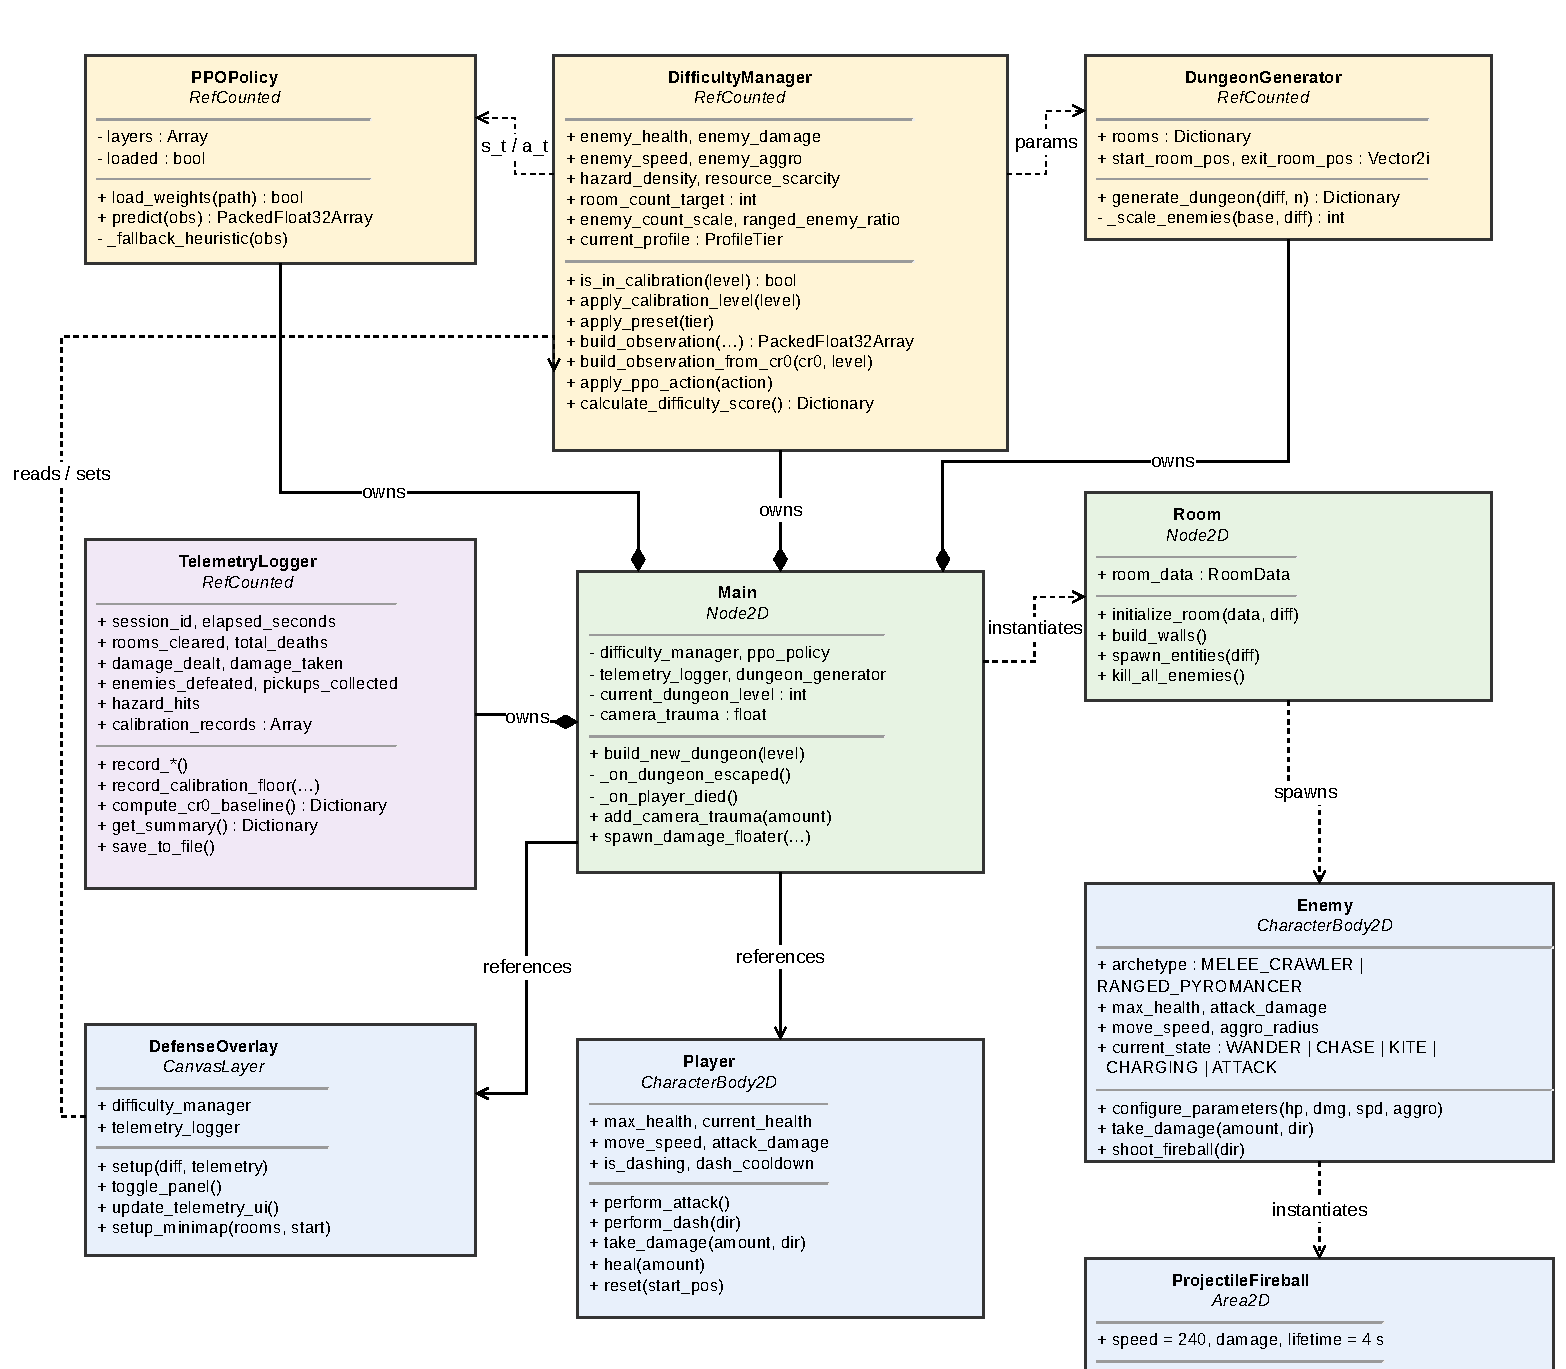
\includegraphics[width=0.98\textwidth]{ThesisFigs/fig_class_diagram}
\caption[UML Class Diagram of the Core Architecture]{UML Class Diagram of the Core Architecture (Mid-1 drawing; \tofill{redraw with TelemetryBackend, SqliteBackend, JsonBackend, ConsentScreen, FloorRating, PauseMenu, GameSettings, SlamShockwave})}
\label{fig:class_diagram}
\end{figure}

\section{Data Design and Telemetry Schema}\label{sec:sqlite_schema_sec}
Since Final-1 the game stores telemetry in an SQLite database, \texttt{user://forge\_telemetry.db}, written by \texttt{SqliteBackend.gd} (godot-sqlite plugin). The schema lives in \texttt{telemetry/schema.sql} (version 2, with migrations) and all SQL statements in \texttt{telemetry/queries.sql}. If the plugin is missing, \texttt{JsonBackend.gd} writes \texttt{user://session\_telemetry.json} instead, and an old JSON history is imported once. Figure~\ref{fig:erd} shows the tables and Table~\ref{tab:sqlite_schema} the main columns.

\begin{figure}[!htbp]
\centering
\begin{tikzpicture}[ent/.style={rectangle, draw=blue!70, fill=blue!6, text width=4.2cm, font=\scriptsize, align=left, inner sep=4pt}, arr/.style={-latex, thick}]
  \node[ent] (s) {\textbf{sessions}\\ \underline{id} \quad install\_id \quad mode\\ policy\_version \quad game\_version\\ consent \quad totals};
  \node[ent, right=1.4cm of s] (f) {\textbf{floors}\\ \underline{id} \quad session\_id (FK)\\ floor\_num \quad phase\\ outcomes \quad 8 settings + 5 mix shares\\ obs\_0..7 \quad action\_0..7\\ frame times \quad perceived\_difficulty\\ manual\_override};
  \node[ent, below=0.8cm of f] (k) {\textbf{kills\_by\_archetype}\\ floor\_id (FK) \quad archetype\_idx \quad count};
  \node[ent, below=0.8cm of s] (v) {\textbf{v\_corpus} (view)\\ floors joined with their session (incl.\ consent flag); read by the Judge};
  \draw[arr] (s) -- node[above, font=\scriptsize]{1 : n} (f);
  \draw[arr] (f) -- node[right, font=\scriptsize]{1 : n} (k);
  \draw[arr, dashed] (f) -- (v);
\end{tikzpicture}
\caption{Entity-relationship diagram of the SQLite telemetry schema (version 2)}
\label{fig:erd}
\end{figure}

\begin{table}[!htbp]
\centering
\caption{Main columns of the SQLite telemetry schema (\texttt{schema.sql}, v2)}
\label{tab:sqlite_schema}
\scriptsize
\begin{tabular}{p{0.15\textwidth}p{0.30\textwidth}p{0.47\textwidth}}
\toprule
\textbf{Table} & \textbf{Column(s)} & \textbf{Meaning} \\
\midrule
sessions & \texttt{id}, \texttt{install\_id} & Session key; random per-installation ID (pseudonymous) \\
sessions & \texttt{mode} & \texttt{adaptive}, \texttt{static} or \texttt{unknown} (a \texttt{bsp} value needs schema v3) \\
sessions & \texttt{consent}, \texttt{policy\_version}, \texttt{game\_version} & Research consent flag; which policy and build produced the data \\
floors & \texttt{floor\_num}, \texttt{phase} & Floor index; \texttt{calibration}, \texttt{adaptive} or \texttt{static} \\
floors & \texttt{completion\_time}, \texttt{deaths}, \texttt{damage\_taken}, \texttt{damage\_dealt} & Outcomes of the floor \\
floors & 8 settings, 5 mix shares, \texttt{enemy\_count\_scale}, \texttt{difficulty\_score} & The configuration $y$ that was played \\
floors & \texttt{obs\_0..7}, \texttt{action\_0..7} & What the policy saw and chose \\
floors & \texttt{frame\_avg\_ms}, \texttt{frame\_p95\_ms}, \texttt{frame\_max\_ms} & Frame times (for NFR-05) \\
floors & \texttt{perceived\_difficulty} & The 1--5 rating, NULL if skipped \\
floors & \texttt{manual\_override} & 1 if the Defense Overlay changed settings; such floors are left out of the Judge corpus \\
kills\_by\_archetype & \texttt{archetype\_idx}, \texttt{count} & Kills per enemy type per floor \\
\bottomrule
\end{tabular}
\end{table}

On the Python side, \texttt{ml\_spike/telemetry\_data/telemetry\_db.py} merges game databases (\texttt{sync\_from\_game\_db}) and returns the Judge's training data; \texttt{export\_telemetry.py} exports a flat CSV, optionally consented sessions only.

\textbf{Data audit (handoff Step 0).} At the time of writing the real data is \textbf{29 consented floors in 3 sessions from one install (one player)}, all rated and all with full settings logged. An older dev database (10 floors, no consent, schema v1) is not used. \tofill{update these counts after syncing the latest playtester databases}

\section{Process and Behavioral Design}

\subsection{Activity Diagram: Complete Game Session Lifecycle}
Figure~\ref{fig:activity_session} details the operational lifecycle of a gameplay session from menu initialization through cold-start calibration to closed-loop adaptive generation.

\begin{figure}[!htbp]
\centering
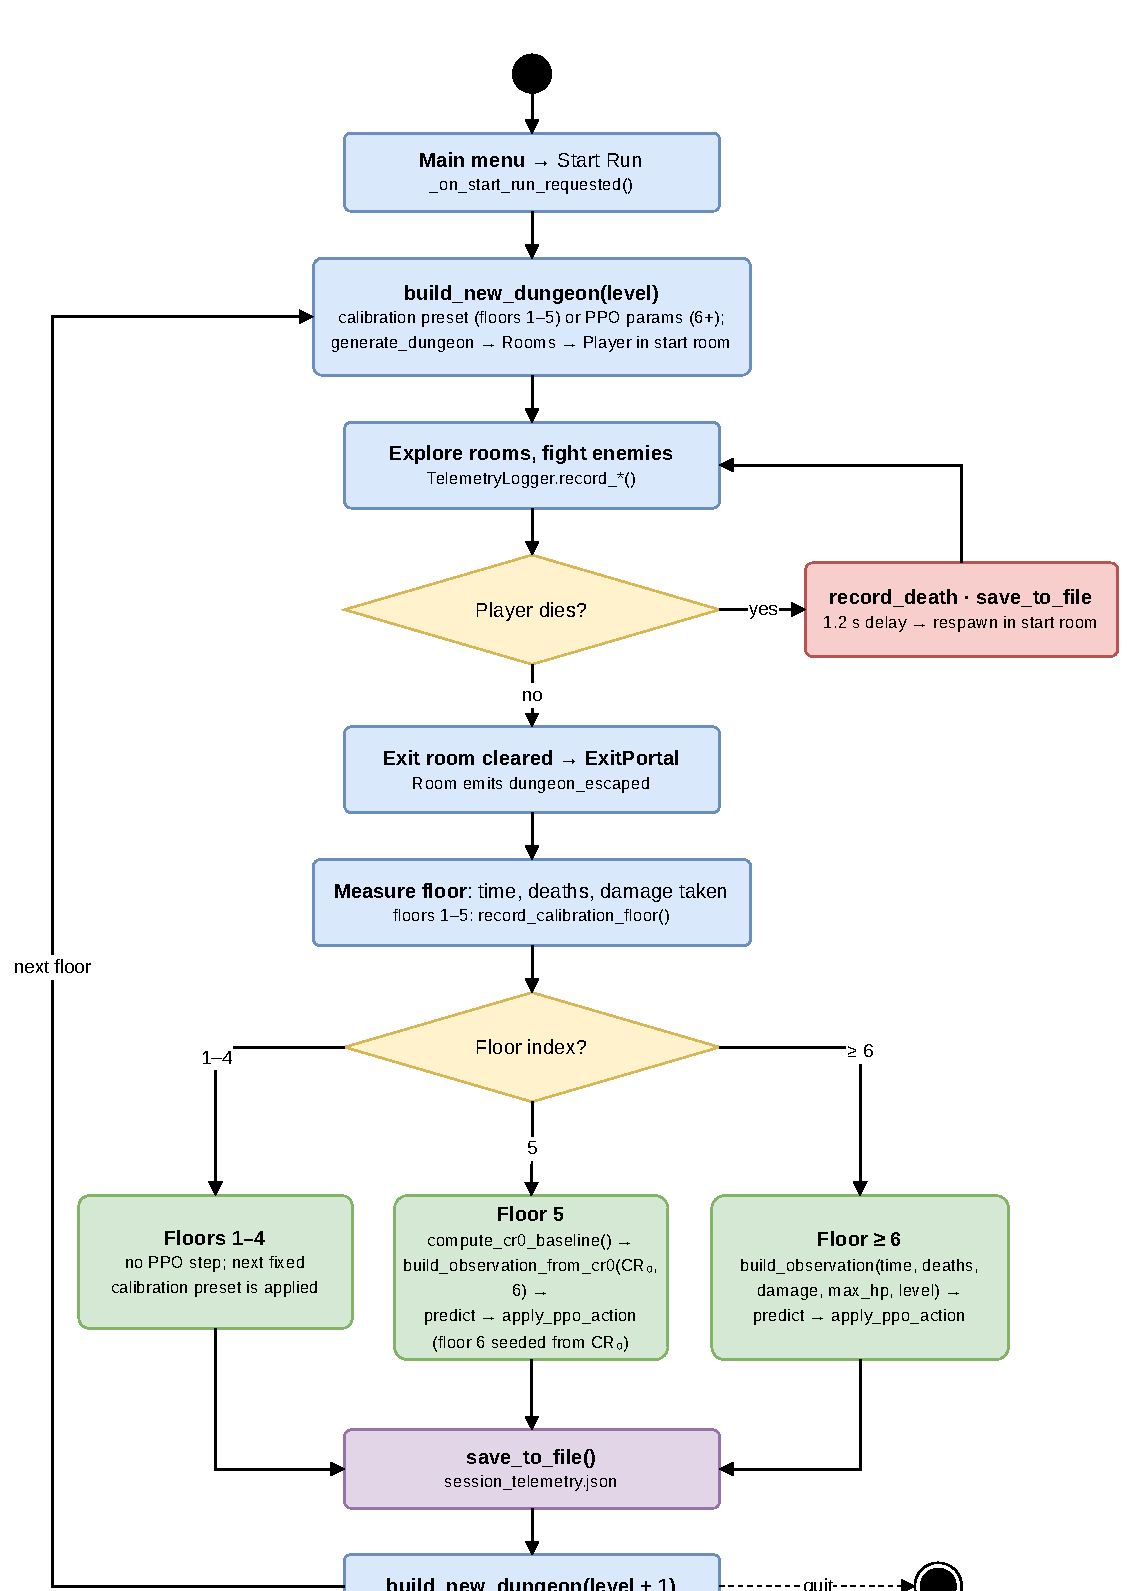
\includegraphics[width=0.65\textwidth, height=0.75\textheight, keepaspectratio]{ThesisFigs/fig_5_8_1_activity_diagram}
\caption{Activity Diagram Illustrating Complete Game Session Lifecycle}
\label{fig:activity_session}
\end{figure}

\subsection{Sequence Diagram: Inter-Floor Telemetry and Adaptation Cycle}
Figure~\ref{fig:seq_diagram} traces the message exchange when the player leaves a floor: calibration floors 1--4 only record telemetry, floor 5 computes $CR_0$ and seeds the first PPO action from the weighted calibration records ($s_0$, Equation~\ref{eq:s0_seed}), and floors 6 and above run one PPO step per floor.

\begin{figure}[!htbp]
\centering
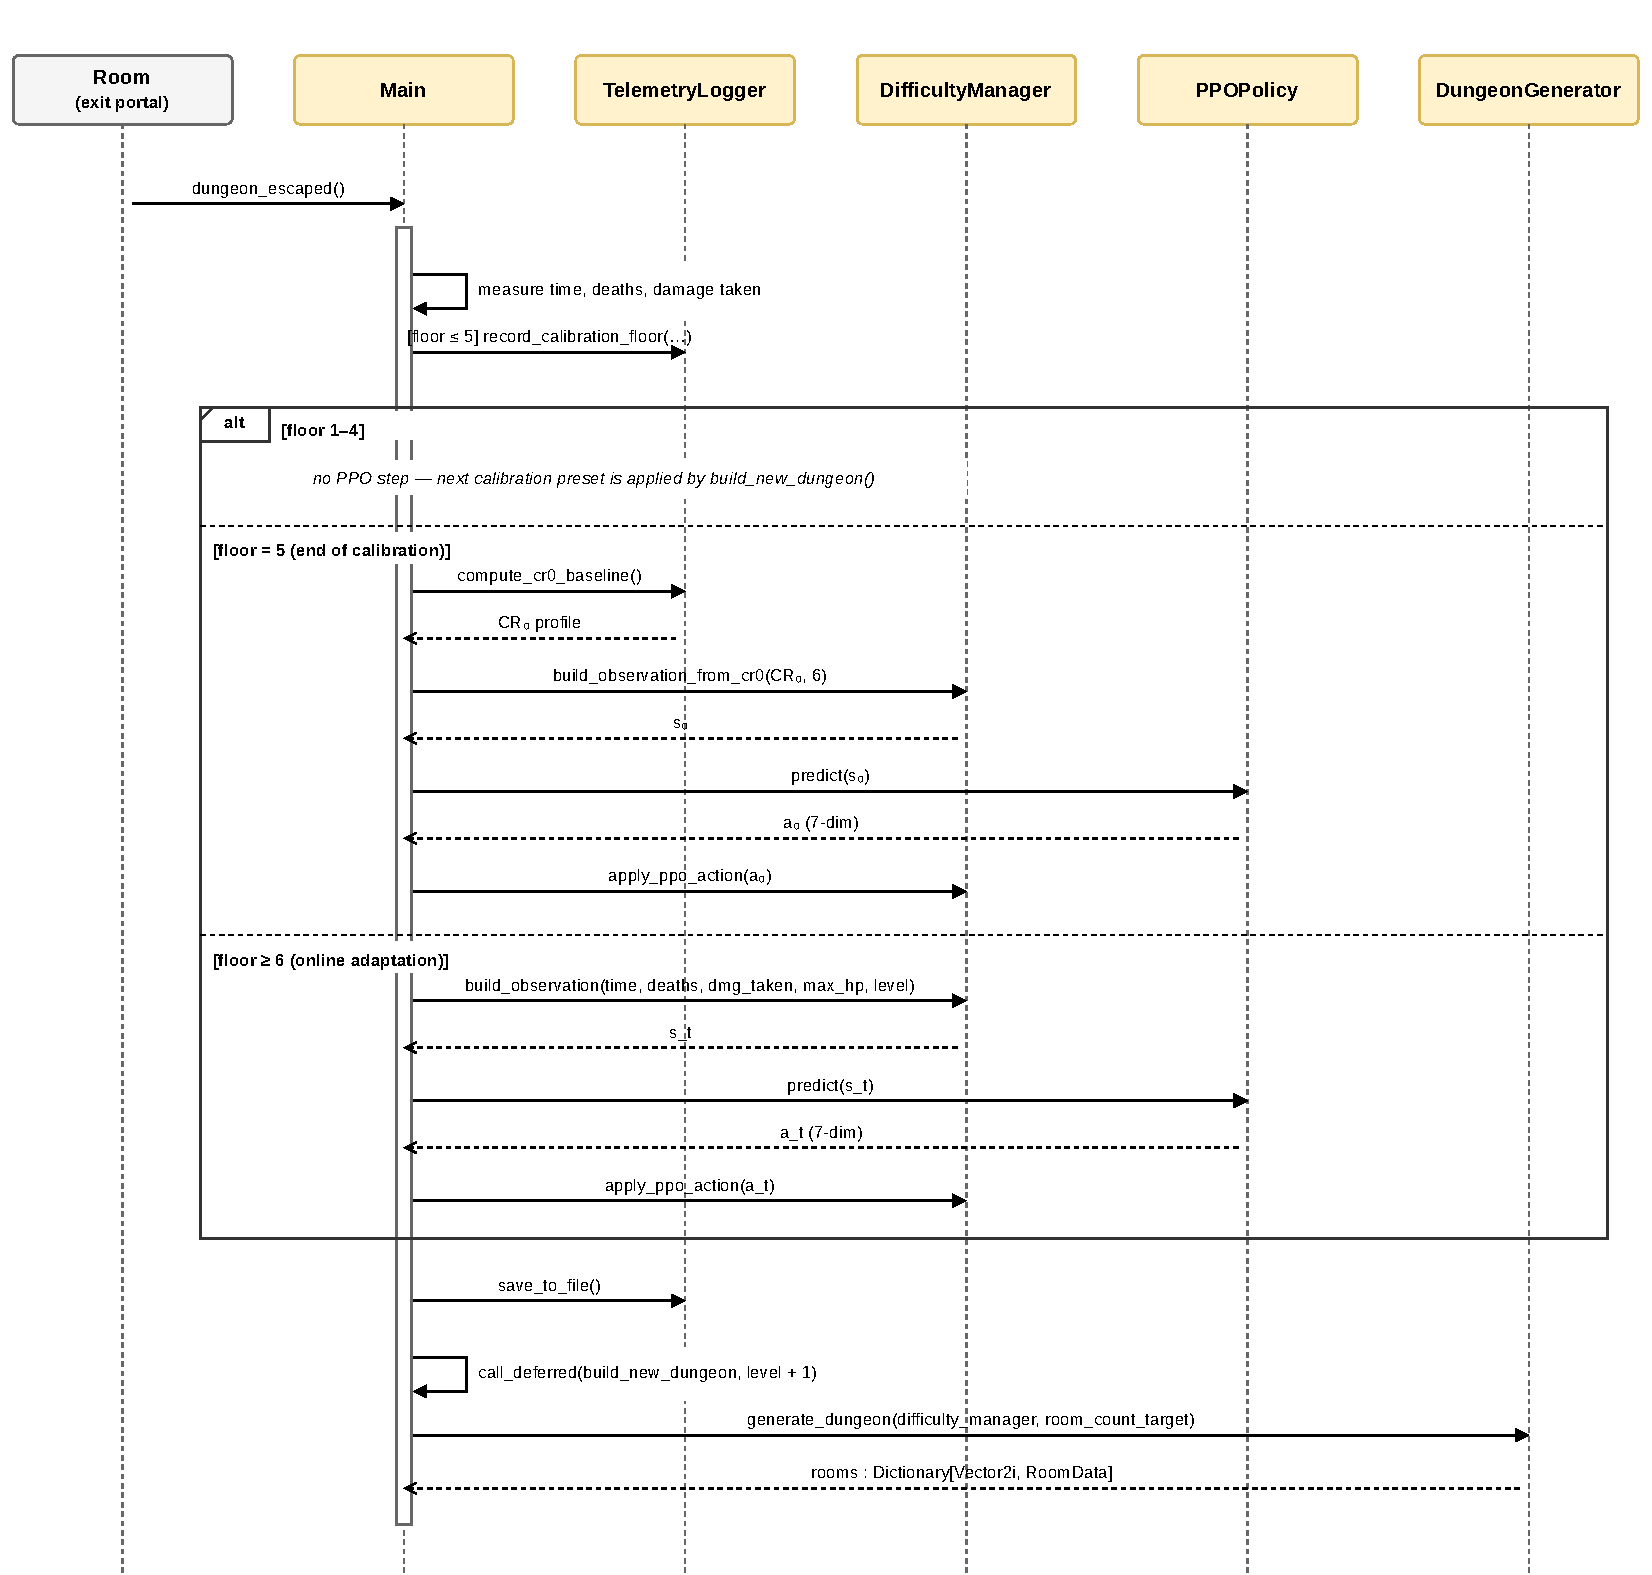
\includegraphics[width=0.98\textwidth]{ThesisFigs/fig_seq_inter_floor_adaptation}
\caption[UML Sequence Diagram of the Inter-Floor Adaptation Step]{UML Sequence Diagram of the Inter-Floor Adaptation Step (\texttt{Main.\_on\_dungeon\_escaped})}
\label{fig:seq_diagram}
\end{figure}

\subsection{State Machine Diagram: Enemy Combat AI}
Figure~\ref{fig:state_enemy} shows the finite state machines governing the two adversary archetypes in \texttt{Enemy.gd}. State changes are driven by the distance $d$ to the player rather than by timers, except for the Pyromancer's $0.5$\,s charge.

\begin{figure}[!htbp]
\centering
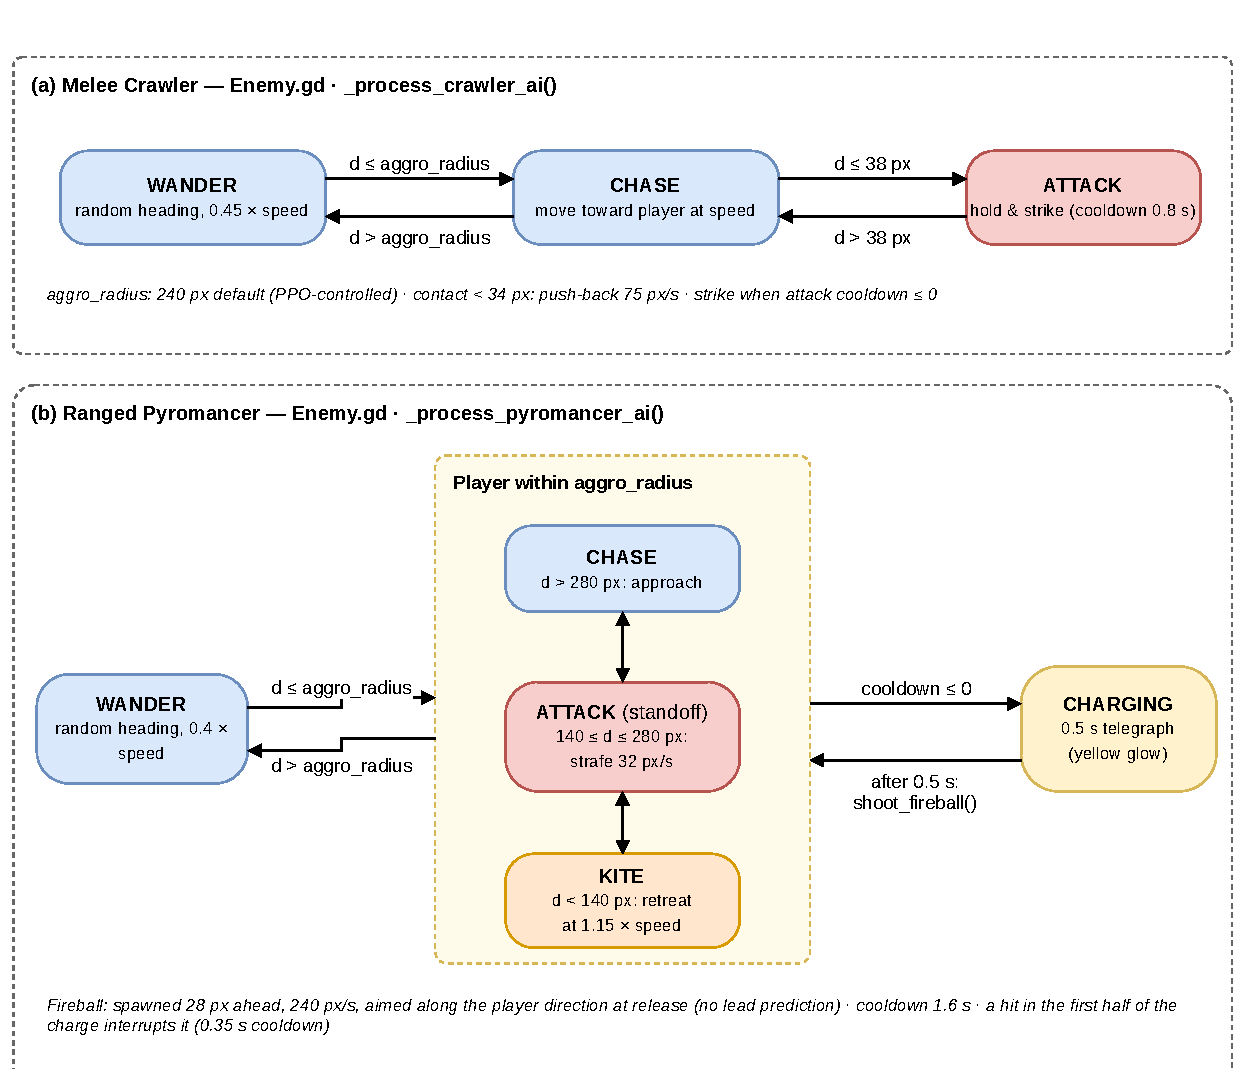
\includegraphics[width=0.85\textwidth]{ThesisFigs/fig_state_enemy_ai}
\caption[Finite State Machines of the Melee Crawler and Ranged Pyromancer]{Finite State Machines of the Melee Crawler and Ranged Pyromancer (\texttt{Enemy.gd}; Mid-1 drawing, the other three archetypes are in Table~\ref{tab:archetypes})}
\label{fig:state_enemy}
\end{figure}

\subsection{The Five Enemy Archetypes}
Table~\ref{tab:archetypes} summarises the five archetypes in \texttt{Enemy.gd}. Each enemy's stats are the floor's base value times its archetype multiplier. The numbers on the right are at the Intermediate preset (HP 60, damage 20, speed 130, aggro 250). Figure~\ref{fig:state_enemy} still shows only the two Mid-1 archetypes and must be redrawn.

\begin{table}[!htbp]
\centering
\caption{Enemy archetypes (\texttt{ARCHETYPE\_MULTIPLIERS} in \texttt{Enemy.gd})}
\label{tab:archetypes}
\scriptsize
\begin{tabular}{p{0.14\textwidth}p{0.17\textwidth}p{0.17\textwidth}p{0.44\textwidth}}
\toprule
\textbf{Archetype} & \textbf{HP / Dmg / Speed $\times$} & \textbf{At Intermediate} & \textbf{Behaviour and telegraph} \\
\midrule
Melee Crawler & 1.0 / 1.0 / 1.0 & 60 / 20 / 130 & Chases inside aggro range; strikes within 38\,px every 0.8\,s. \\
Ranged Pyromancer & 0.75 / 0.9 / 0.92 & 45 / 18 / 120 & Needs line of sight; keeps 140--280\,px away; 0.5\,s yellow telegraph, fireball at 240\,px/s. \\
Heavy Brute & 2.0 / 1.4 / 0.55 & 120 / 28 / 72 & 0.7\,s ground-slam wind-up with a growing red circle; hits within 90\,px; takes only 30\% knockback. \\
Agile Skirmisher & 0.8 / 0.8 / 1.3 & 48 / 16 / 169 & Orbits at 120--160\,px; 0.2\,s cyan aim line, then a fast lunge and retreat. \\
Swarmer & 0.35 / 0.45 / 1.15 & 21 / 9 / 150 & One spawn slot is a pack of 3 that approach from the flanks and bite. \\
\bottomrule
\end{tabular}
\end{table}
In the exit room, when enemy health is 85 or more, one Brute becomes an ``apex champion'' ($\times1.7$ HP, $\times1.25$ damage). This happens on Floor 5 and also on any adaptive floor with high health, and the simulator does not model it (Section~\ref{sec:limitations}).
